\documentclass[twocolumn,nofootinbib]{revtex4-1}
\usepackage{graphics}
\usepackage[caption=false]{subfig}
\usepackage{amsmath}
\usepackage{hyperref}
\usepackage{amssymb}
\usepackage{color}
\usepackage{epsfig}
\usepackage{latexsym}
\usepackage{tensor}
\usepackage{float}
\usepackage{multirow}
%\usepackage{wasysym}
\usepackage{comment}
%\usepackage{graphicx}
%\usepackage{psfrag}

\graphicspath{{poster/figures/}}

%\newcommand{\gw}{gravitational wave }
%\newcommand{\gws}{gravitational waves }
\newcommand{\subgw}{_{\textrm{\scriptsize{GW}}}}
\newcommand{\ee}[1]{\!\times\!10^{#1}}
\newcommand{\prob}{{\rm Pr}}
\newcommand{\grbrate}{{{\mathcal R}_{\mathrm{grb}}}}
\newcommand{\cbcrate}{{{\mathcal R}}}
\newcommand{\diff}{{\mathrm d}}
\newcommand{\rhostar}{{\rho^*}}
\newcommand{\dhor}{{\mathcal D}_{\mathrm{hor}}}

\def\imbh#1{intermediate mass black hole#1(IMBH#1)\gdef\imbh{IMBH}}
\def\smbh#1{supermassive black hole#1(SMBH#1)\gdef\smbh{SMBH}}
\def\bbh#1{binary black hole#1 (BBH#1)\gdef\bbh{BBH}}
\def\bns#1{binary neutron star#1 (BNS#1)\gdef\bns{BNS}}
\def\bh#1{black hole#1 (BH#1)\gdef\bh{BH}}
\def\ns#1{neutron star#1 (NS#1)\gdef\ns{NS}}
\def\gw#1{gravitational wave#1 (GW#1)\gdef\gw{GW}}
\def\sn#1{core-collapse supernova#1 (CCSN#1)\gdef\sn{CCSN}}
\def\pnw#1{post-Newtonian#1 (PN#1)\gdef\pnw{PN}}
\def\eos#1{equation of state#1 (EOS#1)\gdef\eos{EOS}}
\def\grb#1{gamma-ray burst#1 (GRB#1)\gdef\grb{GRB}}
\def\sgrb#1{short gamma-ray burst#1 (sGRB#1)\gdef\sgrb{sGRB}}
\def\electro#1{electromagnetic#1 (EM#1)\gdef\electro{EM}}
\def\amr#1{adaptive mesh refinement#1 (AMR#1)\gdef\amr{AMR}}
\def\isco#1{innermost stable circular orbit#1 (ISCO#1)\gdef\isco{ISCO}}
\def\cwb#1{Coherent WaveBurst#1 (CWB#1)\gdef\cwb{CWB}}
\def\mweg#1{Milky Way Equivalent Galaxy#1 (MWEG#1)\gdef\mweg{MWEG}}
\def\snr#1{signal-to-noise ratio#1 (SNR#1)\gdef\snr{SNR}}

\newcommand{\red}[1]{{\color{red}{#1}}}
\newcommand{\about}[1]{{\color{blue}{[THIS SECTION: #1]}}}
\newcommand{\add}[1]{{\color{magenta}{[TO INCLUDE: #1]}}}
\newcommand{\JC}[1]{{\color{magenta}{[[JC #1]]}}}
\newcommand{\placeholder}[2]{{\color{red}{[PLACEHOLDER](#1):}}{\color{red}{[}}#2{\color{red}{]}}}
\providecommand{\todo}[1]{{\color{red}$\blacksquare$~\textsf{[TODO: #1]}}}


\def\pasp{Publications of the Astronomical Society of the Pacific}
\def\mnras{Monthly Notices of the Royal Astronomical Society}
\def\aap{Astronomy and Astrophysics}


%%%%%% Useful for draft editing
\usepackage{soul} 
\usepackage{ulem} \normalem 
\newcommand{\ec}[1]{{\noindent\color{red}{\it [[#1]] }}}
\newcommand{\laura}[1]{{\color{blue}{#1}}}
\newcommand{\LC}[1]{{\color{red}{[[LC #1]]}}}
\newcommand{\AB}[1]{{\color{blue}{[[AB #1]]}}}
\newcommand{\highlight}[1]{\colorbox{yellow}{#1}}
\newcommand{\simgt}{\mbox{$^{>}_{\sim}$}}

\begin{document}

\title{Constraints On Short, Hard Gamma-Ray Burst Beaming Angles From
Gravitational Wave Observations}
\author{James Clark, Ik Siong Heng, Martin Hendry}
\date{\today}

\begin{abstract}
\dots
\end{abstract}

\maketitle

\section{Introduction}

\about{Intro with also many words taken from search plans}

Extremely energetic bursts of gamma-rays from cosmological sources are observed by orbiting satellite detectors at a rate of about one per day. These extra-galactic events are generally referred to as GRBs.
GRBs are generally associated with systems which are also expected to be \gw{} sources: compact binary coalescences for \sgrb{}, with gamma-ray duration $<\!2\,$s and harder spectra [ref].

The detection of a GW signal in coincidence with a GRB would provide tremendous insight in the  astrophysics of these systems.
A merger signal associated to a short GRB would confirm the compact binary merger nature of the engine and allow for measurements of the binary components masses and spins, as well as constraints on the beaming angles and the neutron star equation of state.
However, it is only the observation of a GW signal that will conclusively show that the progenitor is a binary merger. While the merger scenario is preferred and at least one NS is required, both NS-NS and NS-BH progenitors are possible; GW observations will allow us to determine which of these it is. A population of GW-GRB observations will allow us to measure the fraction of GRBs associated with each progenitor type. The degeneracy between distance and inclination angle means that it will be difficult to measure the GRB beaming angle based on measurement of a single system. However, with observations of a population of binary merger sources, with and without GRB counterparts, we can constrain the average opening angle.   
A collection of joint short GRBs with redshift and GW measurements will also enable a relatively systematics-free measurement of the Hubble parameter at low redshift, which would provide constraints on cosmological models.

%It is common in the literature to draw inferences on the rate of binary
%coalescence $\cbcrate$, given some estimate for the beaming angle $\theta$ and
%the observed rate of \sgrb{s} $\grbrate$.  
In this work, we investigate what
statements can \emph{currently} be made on the beaming angle itself using the
upper limits placed on $\cbcrate$ from all-sky, all-time \gw{} searches and
explore the potential for direct inference of \sgrb{}  beaming angles in the
advanced detector era.

In this article, we first discuss the relationship between short gamma-ray bursts
and compact binary coalescences. In particular, we will focus on binary neutron 
star inspirals as the widely accepted progenitor for short gamma-ray bursts.
We then present our method for robustly inferring the jet opening angles of 
short gamma-ray bursts, using only gravitational wave observations. We 
demonstrate our method by assuming the nominal number of gravitational
wave signals observed from binary neutron star inspirals expected for
Advanced LIGO and Advanced Virgo in 2016 and 2022 as defined in [ref]. 
We also show that our approach can be used to place restrictions on the
short gamma-ray burst jet opening angle if there are no detections.
Finally, we conclude with a discussion on the implications of our work
as well as possible avenues for further extension of the work presented
here.

%\section{Inferring The sGRB Beaming Angle From Rate Measurements}
\section{Short gamma-ray bursts and compact binary coalescences}
\label{sec:sgrbs}

\about{Some description of BNS and how they are likely progenitors of short
gamma-ray bursts (This section describes our model and how sGRBs relate to BNS, currently with text taken from LVC search plans}

It is widely believed that compact binary coalescencesare the progenitors of \sgrb{s} [ref]. 
Observations of \sgrb{s} indicate that they are likely to result from mergers of binary systems consisting of  two neutron stars (\bns{}) or a neutron star and stellar mass ($< 10$ solar mass) black hole (NS-BH). 
At full sensitivity, they are potentially observable by advanced GW detectors to $\sim 400\,$Mpc for NS-NS or $\sim 1\,$Gpc for NS-BH at a rate of $\sim 1\,$yr$^{-1}$ for each~\cite{MetzgerBerger, Clark:2014ut}. 
It is worth noting that at galactic or near-galactic distances, soft gamma-ray repeater (SGR) hyperflares can also be observed as a \sgrb{}. 
These SGR hyperflares are the likely explanations for GRB 070201 and GRB 051103 since compact binary coalescences at the distance of their host galaxies were excluded with greater than $90\%$ confidence as progenitors of these \sgrb{s} [refs]. 

Given the link between \sgrb{s} and compact binary coalescences, it is interest
to ask whether the \sgrb{} beaming angle can be inferred from \gw{}
observations.  For example, a joint \gw{}-\grb{} observation could, in
principal, constrain the beaming angle by directly measuring the orbital
inclination of the system via \gw{s}.  As discussed
in~\cite{0004-637X-809-1-53}, however, the likely low \snr{} of such an
observation and the degeneracy between orbital inclination and distance suggest
that a comparison of the populations of observed \sgrb{s} and \bns{} mergers may
be more promising.   Motivated by the study in~\cite{2013PhRvL.111r1101C}, we
note that if the \sgrb{} population posseses a distribution of beaming angles
then the \emph{observed} rate of \sgrb{s} is related to the rate of \bns{}
coalescence $\cbcrate$ via,
%
\begin{equation}\label{eq:rate2angle}
    \grbrate = \epsilon\cbcrate \left \langle 1-\cos \theta \right \rangle,
\end{equation}
%
where angled brackets $\langle \rangle$ indicate the population mean and
$\epsilon$ is the probability that a binary coalescence results in an observed
\sgrb{}.  In this work, we assume
$\grbrate=10$\,Gpc$^{-3}$\,yr$^{-1}$~\cite{nakar-2007,Dietz11} and we shall
refer to $\epsilon$ as the \sgrb{} \emph{efficiency}.  Generally, the efficiency
with which \bns{} mergers produce \sgrb{s} is unknown but will depend on a
variety of progenitor physics.  We note that efforts are underway [Pannarale] to
characterize systems which are likely to yield \sgrb{s}.  Combining this
knowledge with measurements of the binary parameters of of a population of joint
\gw{}-\electro{} observations could be used to constrain $\epsilon$.  In this
work, we will make no attempt to characterize $\epsilon$ and we simply aim to
provide a framework which allows one to incorporate various levels of
assumptions (or ignorance) regarding its value.   

If the \sgrb{} population has a distribution of beaming angles, as would seem
likely from \electro{} observations, characterizing the relative rates of
\sgrb{} and \bns{} coalescence will inform us as to the mean of that population,
$\langle \theta \rangle$.  To explore this point further we construct a simple
Monte-Carlo simulation to study the effect on the relative rates of \sgrb{s} and
\bns{} mergers.  We arrange the following toy problem:
%
\begin{enumerate}
    \item Set the number of `observed \grb{s} to zero: $N_{\mathrm{GRB}}=0$.
    \item Draw $N_{\mathrm{bns}}$ values of orbital inclination $\iota$ from a
        distribution which is uniform in $\cos \iota$ in the range $[0,1]$.
    \item For each value of $\iota$, draw a value for the beaming angle
    $\theta$, from some distribution with finite width and limited to the range
$(0,90]^{\circ}$.  
    \item If $\iota<\theta$ then this combination of orbital inclination and
        beaming angle would result in an observable \grb{}, so increment
        $N_{\mathrm{GRB}}$
\end{enumerate}
%
Such a simulation allows us to study the ratio of the number of observed
\grb{s} to the total number of \bns{} mergers $N_{\mathrm{GRB}}/
N_{\mathrm{bns}}$.  Since it is the comparison of the rates of these events
which informs our inference on $\theta$,  studying the ratio $N_{\mathrm{GRB}}
/N_{\mathrm{bns}}$ provides some intuition as to the effect and features of
various $\theta$ distributions.  Figure~\ref{fig:thetapop} plots this ratio as a
function of various truncated normal distributions to demonstrate the effect of
shifting the mean and scaling the width of the distribution. Points along the
$x$-axis correspond to different choices of the distribution width
$\sigma_{\theta}$ and the
separate curves correspond to different choices of the distribution mean
$\langle \theta \rangle$.  Let us denote this truncated normal distribution
${\mathcal N}(\langle \theta \rangle, \sigma_{\theta})$.  We
stress here that such $\theta$ distributions are \emph{not} intended to
represent the true distribution; they are merely intended to easily
demonstrate the qualitative effects of different $\theta$ distributions on the
ratio $N_{\mathrm{GRB}}/N_{\mathrm{bns}}$.

Figure~\ref{fig:thetapop} reveals that a population of \sgrb{} beaming angles
with a large mean but narrow width is, on the basis of rate measurements,
indidstinguishable from a population of \sgrb{} beaming angles with a small mean
and large width.  Consider, for example, the ratio for the $N(15,8)$ beaming
angle population. 
 

\begin{figure}
\centering
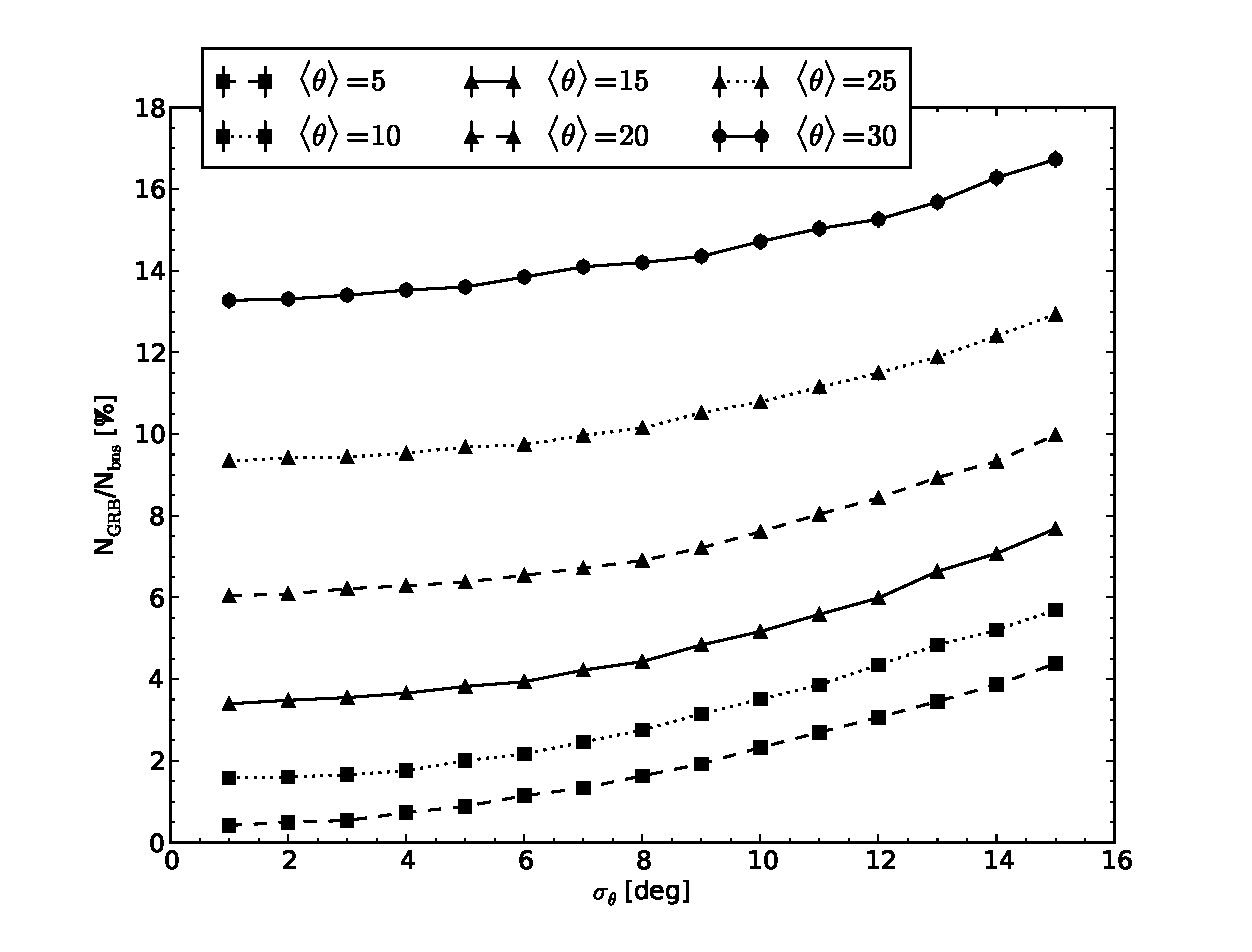
\includegraphics[width=\linewidth]{theta_dist_grbfrac.eps}
\caption{\label{fig:thetapopulation} Expected relative
numbers of observed GRBs and binary coalescences for different distributions
on the GRB beaming angle.  Lines in the figure correspond to jet angle
population means, while the $x$-axis shows the width of the distribution.  All 
distributions are Gaussian, truncated at $(0, 90]$ degrees.\label{fig:thetapop}}
\end{figure}


\section{From Rates To Beaming Angles}

In this section, we discuss our approach to estimating the \sgrb{} beaming
angle based on the binary neutron star inspiral rate, estimated through a number
of \gw{} observations of \bns{} coalescence. We demonstrate the approach by
considering plausible detection scenarios in aLIGO.  Our ultimate goal is to
develop a generic approach that folds in uncertainties in in the binary neutron
star inspiral rate and our ignorance about the probability with which binary
neutron star inspirals actually result in \sgrb{s}.
%
An overview of the general method is as follows:

\begin{enumerate}
    \item Estimate the posterior probability distribution on the \bns{} merger rate
    in the local Universe from a number of observed gravitational wave signals
    and our knowledge of the sensitivity of the detectors.  We construct a joint
    posterior distribution on the \bns{} rate and the (unknown) probability
    $\epsilon$ that a given merger results in a \sgrb{}.
\item Use equation~\ref{eq:rate2angle}, which relates the \bns{} merger and
    \sgrb{} rates via the geometry of the beaming angle, to transform the rate
    posterior probability to a posterior probability on the mean short gamma-ray
    burst beaming angle.
\item Marginalize over $\epsilon$. We choose to consider $\epsilon$ a nuisance
    parameter because, to date, there is no accurate estimate of this parameter
    and it is not the main focus of our analysis. 
\end{enumerate}


\subsection{Constructing The Rate Posterior}
\label{sec:rate_posterior}
%   Gregory's book, `Logical Data Analysis For The Physical Sciences' has an entire
%   chapter (\S 14) devoted to `Bayesian Inference With Poisson Sampling'.  This
%   seems to match our problem rather well.  In particular, he derives expressions
%   for a Poisson rate posterior in \S 14.3, `Signal + known background' and \S
%   14.4, `Analysis of ON/OFF measurements' (``we want to infer the source rate, s,
%   when the background rate, b, is imprecisely measured'').
%
%It's tempting to jump straight into the On/off measurement stuff in \S~14.4 of
%Gregory, where the construction of the rate posterior includes the raw
%measurements of background rate.  I actually think this over-complicates things;
%if we wanted to do follow that procedure, we have to figure out the expected FAR
%for a given size of template bank etc.  There's a pretty well-established
%procedure for measuring this number: time-slides.  In fact, we don't even have
%to do any analysis.  Figure 3 (left panel) from the observing scenarios paper
%tells us everything we need to know.  Specifically, the following sentance has
%the information we need:

Our goal is to infer the posterior probability distribution for the mean \sgrb{}
beaming angle $\theta$ from \gw{} constraints on the rate of \bns{} coalescence
$\cbcrate$.  The core ingredient to the analysis then, is the posterior
probability distribution on the coalescence rate $p(\cbcrate|D,I)$, where $D$
represents some \gw{} observation and $I$ denotes other unenumerated prior
information.   To begin we will demonstrate how $p(\cbcrate|D,I)$ may be
constructed given a variety of the projected observation scenarios using aLIGO
which are described in~\cite{ade_prospects}.  Later, in
section~\ref{sec:beaming_limits} where we extend the analysis to place upper
limits on $\theta$ from the initial detector era, we consider the rate posterior
yielded by previous \gw{} analyses.

To form the posterior on the coalescence rate, we begin by constructing the
posterior on the \emph{signal} rate.  Note that these are not identical since
only those \bns{} mergers which occur within a certain range yield a detectable
signal.  Assume we have a data analysis pipeline (e.g.,
{\tt FINDCHIRP}~\cite{2012PhRvD..85l2006A}) which, when applied to the data from
our instrument, results in discrete `events' which are characterized by network
signal-to-noise ratio $\rho_c$ and which correspond to the potential
detection of an inspiral \gw{} signal from \bns{} coalescence.  The measured
rate $r$ of these events consists of two components, one due to the signals of
interest $s$, and the other a background rate $b$, which arises due to random
chance and, more importantly, instrumental and terrestrial disturbances:
%
\begin{equation}
r = s + b
\begin{cases}
s = \text{signal rate} \\
b = \text{background rate}.
\end{cases}
\end{equation}
%
Typically for an all-sky, all-time analysis, a threshold $\rho_c\geq 12$ is
applied to the events arising from the pipeline such that
$b=10^{-2}$\,yr$^{-1}$~\cite{ade_prospects}.  Since the background rate $b$ is
known then, we are just left with the problem of inferring the signal rate $s$.
Assuming a uniform prior on $s$ and a Poisson process underlying the events, it
may be shown (e.g.,~\cite{2010blda.book.....G}) that the posterior for the
signal rate, given a known background rate $b$ and $n$ events observed over a
time period $T$ is,
%
\begin{equation}
p(s|n,b,I) = C \frac{ T\left[(s+b)T\right]^n e^{-(s+b)T}}{n!},
\end{equation}
%
where,
\begin{eqnarray}
C^{-1} & = &\frac{e^{-bT}}{n!} \int_0^{\infty}\diff(sT)(s+b)^n T^n e^{-sT}\\
& = & \sum_{i=0}^n \frac{ (bT)^i e^{-bT}}{i!}.
\end{eqnarray}
%
Finally, we can transform the posterior on the \emph{signal} rate to the
underlying \emph{coalescence} rate via our knowledge of the sensitivity of the
\gw{} analysis.  In particular,  the signal detection rate is simply the product
of the intrinsic coalescence rate $\cbcrate$ and the number of \bns{} mergers
which would result in a \gw{} signal with $\rho_c\geq12$.   Expressing the
binary coalescence rate in terms of the number of mergers per \mweg{}, per year
then we require the number of galaxies $N_{\mathrm{G}}$ which may be probed by
the \gw{} analysis.  At large distances, this is well approximated at large
distances by~\cite{rates_paper},
%
\begin{equation}
    N_G = \frac{4}{3} \pi \left( \frac{\dhor}{\textrm{Mpc}}
\right)^3 (2.26)^{-3} (0.0116),
\end{equation}
%
where $\dhor$ is the horizon distance; the distance at which an
optimally-oriented \bns{} merger yields $\rho_c\geq12$, the factor of 2.26
results from averaging over sky-locations and orientations and $1.16\times
10^{-2}$\,Mpc$^{-3}$ is the extrapolated density of \mweg{} in space.

Finally, the posterior on the binary coalescence rate $\cbcrate$ is obtained from
a trivial transformation of the posterior on the signal rate $s$,
%
\begin{eqnarray}
    p(\cbcrate|n,T,b,\dhor) & = & p(s|n,T,b) \left|\frac{\diff s}{\diff \cbcrate}\right| \\
                                   & = & N_G(\dhor)p(s|n,T,b).
\end{eqnarray}
%
We see then that in this approach, the rate posterior depends only on the number
of signal detections $n$, the observation time $T$, the background rate $b$ and
the horizon distance of the search $\dhor$.  It is precisely these quantities
that comprise the detection scenarios outlined in~\cite{ade_prospects}.  Before
constructing expected rate posteriors, let us outline the transformation from
rate to beaming angle.

\subsection{Constructing the beaming angle posterior}
Inferences of the GRB beaming angle are made from the posterior probability
density on the beaming angle $p(\theta|D,I)$ where, as usual $D$ indicates some
set of observations and $I$ unenumerated prior knowledge.  Our goal then, is to
transform the measured posterior probability density on the rate $\cbcrate$ to a
posterior on the beaming angle.
%
First, note that we can express the joint distribution $p(\theta, \epsilon|D,I)$
as a Jacobian transformation of the joint distribution $p(\cbcrate,
\epsilon|D,I)$:
\begin{equation}
p(\theta,\epsilon) = p(\cbcrate,\epsilon)
\left\lvert\left\lvert
\frac{\partial(\cbcrate,\epsilon)}{\partial(\theta,\epsilon)}
\right\rvert\right\rvert,
\end{equation}
%
where we have dropped conditioning statements for notational convenience.  The
Jacobian determinant is can be  computed from equation~\ref{eq:rate2angle}.  It
is then straightforward to marginalize over $\epsilon$ to yield the posterior
on $\theta$ itself:
%
\begin{eqnarray}
    \label{eq:beam_posterior}
    p(\theta) & = & \int_{\epsilon} p(\theta,\epsilon)~\diff \epsilon\\
              & = & \int_{\epsilon} p(\cbcrate,\epsilon)
    \left\lvert\left\lvert
    \frac{\partial(\cbcrate,\epsilon)}{\partial(\theta,\epsilon)}
    \right\rvert\right\rvert~\diff \epsilon \\
              & = & \frac{2\grbrate \sin
\theta~p(\cbcrate)}{(\cos\theta-1)^2}\int_{\epsilon}
\frac{p(\epsilon)}{\epsilon} ~\diff \epsilon,
\end{eqnarray}
%
where we have assumed $\epsilon$ and $\cbcrate$ are logically independent such
that,
\begin{equation}
p(\epsilon,\cbcrate) = p(\epsilon|\cbcrate)p(\cbcrate) = p(\epsilon)p(\cbcrate).
\end{equation}
%
It is important note here that the entire procedure of deriving the jet angle
posterior is completely independent of the approach used to derive the rate
posterior. In the preceeding section we adopted a straightforward Bayesian
analysis of a Poisson rate which is amenable to a simple application of plausible
future detection scenarios; there is no inherent requirement to use that method
to derive the rate posterior.

Given the posterior on the rate $p(\cbcrate)$ then, the final ingredient in this
approach is the specification of some prior distribution for $\epsilon$.  In
this work, we will present results using three different priors:
%
\begin{description}
\item [Delta-function] $p(\epsilon) = \delta(\epsilon=0.5)$;
        the probability that \bns{} mergers yield \sgrb{s} is known to be 50\%
        exactly.

\item [Uniform] $p(\epsilon)=U(0,1)$;
        the probability that \bns{} mergers yield \sgrb{s} may lie anywhere
    $\epsilon \in (0,1]$ with equal support in that range. 

    \item [Jeffreys] $p(\epsilon)=\beta(\frac{1}{2},\frac{1}{2})$; treating the
        outcome of a \bns{} merger as a Bernoulli trial in which a \sgrb{}
        constitutes `success' and $\epsilon$ is the probability of that success,
        the least informative prior, as derived from the square root of the
        determinant of the Fisher information for the Bernoulli distribution, is
        a $\beta$-distribution with shape parameters $\alpha=\beta=\frac{1}{2}$.
\end{description}

%   \begin{figure}%[ht]
%   \centering
%   {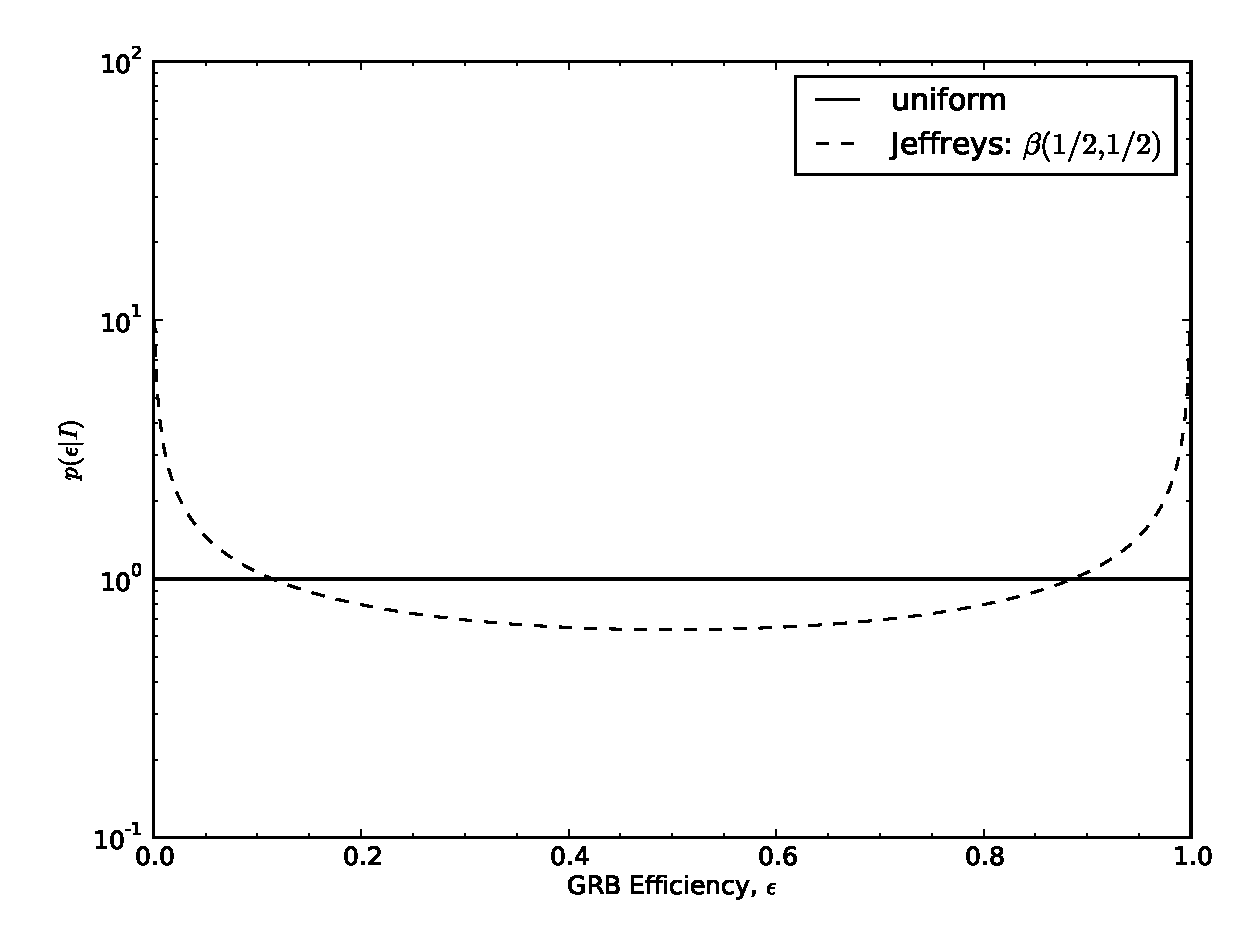
\includegraphics[width=\linewidth]{efficiency_prior.eps}}\label{fig:priors}
%   \caption{Priors}
%   \end{figure}

\subsection{A Note On Implementation}
Rather than directly evaluating the beaming angle posterior in
equation~\ref{eq:beam_posterior} we choose to sample points from the posterior
using a Markov-Chain Monte-Carlo algorithm, implemented using the python package
{\tt EMCEE}~\cite{2013PASP..125..306F}.  Points are sampled from the joint
distribution $p(\theta,\epsilon)$, where equation~\ref{eq:rate2angle} is used to
derive the corresponding value of $\cbcrate$ for a given $(\theta,\epsilon)$.
We then obtain the marginal distribution $p(\theta)$ via kernel density
estimation (KDE) of the $\theta$-samples.  The mode of the KDE yields the
maximimum a posteriori (MAP) estimate for the measurement and the upper and
lower bounds are found from the 95\% confidence interval around the median of
the samples.

\section{Prospects For Beaming Angle Constraints With aLIGO} We now demonstrate
the derivation of the rate posterior $p(\cbcrate)$ and the subsequent
transformation to the beaming angle posterior $p(\theta)$.  We consider four
\gw{} observation scenarios with aLIGO based on the work
in~\cite{ade_prospects}.  An observing scenario essentially consists of an epoch
of aLIGO operation, which defines an expected search sensitivity (i.e., \bns{}
horizon distance $\dhor$) and observation time $T$; as well as an assumption on
the rate of \bns{} coalescence in the local Universe $\cbcrate$.  Each observing
scenario ultimately results in an expectation for the number of observed \gw{s}
from \bns{} coalescence. For this study, we consider two operation epochs: the
2016 and 2022+ scenarios described in~\cite{ade_prospects} and we assume the
`realistic rate' for $\cbcrate$ as described in~\cite{rates_paper}.

Our first goal is to establish the expected number of detections in each
scenario. Given the observation time and horizon distance of the observation
epoch we first compute the 4-volume accessible to the analysis,
%
\begin{equation}
    \label{eq:search_volume}
    V_{\mathrm{search}} = \frac{4}{3}\pi \left(\frac{\dhor}{2.26}\right)^3 \times \gamma T,
\end{equation}
%
where the factor 2.26 arises from averaging over source sky location and
orientation, $T$ is the observation time and $\gamma$ is the \emph{duty cycle}
for the science run.  Following~\cite{ade_prospects}, we take $\gamma=0.5$.
Where there is a range in the horizon distances quoted in~\cite{ade_prospects}
to account for uncertainty in the sensitivity of the early configuration of the
detectors, we use the arithmetic mean of the lower and upper bounds on when
computing the search volume. Table~\ref{table:scenarios} lists the details of
each observing scenario.


\begin{table}
\centering
\begin{tabular}{l c c c c c }
\toprule
Epoch & $T$ & $\dhor$ &
$\langle V_{\mathrm{search}}\rangle$ & $\cbcrate$ & $n$ \\
 & [yr] & [Mpc] & [Mpc$^3$yr] &  [Mpc$^{-3}$yr$^{-1}$] \\
\colrule
2016 & 0.5 & 80--120 & $1.05\times10^6$ & $10^{-6}$ & 1.3 \\
%2016 & 0.5 & 80--120 & $1.05\times10^6$ & $10^{-5}$ & 13 \\
2022+ & 1 & 200 & $4\times10^7$ & $10^{-6}$ & 40 \\
%2022+ & 1 & 200 & $4\times10^7$ & $10^{-5}$ & 400 \\
\botrule
\end{tabular}
\caption{Advanced detector era observing scenarios considered in this work.  $T$
is the expected duration of the science run and $\dhor$ is the BNS
horizon distance for the sensitivity expected to be acheived at the given epoch.
$\langle V_{\mathrm{search}}\rangle $ is the sensitive volume of the search,
where the angled brackets $\langle \rangle$ indicate averaging over the range
in horzizon distance, $\cbcrate$ is the assumed BNS coalescence rate and
$n$ is the expected number of \gw{} detections.  Note that the
quoted search volume accounts for a network duty cycle of $\sim 50\%$.
Full details may be foud in~\cite{ade_prospects}.\label{table:scenarios}}
\end{table}
%

\subsection{Posterior Results}
Figure~\ref{fig:aligorate} shows the rate posteriors resulting from the
observations described in table~\ref{table:scenarios} for the expected early
aLIGO sensitivity in the 2016 epoch (broad, solid curve) and the nominal design
sensivity (narrow, dashed curve), using the `realistic' rate
$\cbcrate=10^{-6}$\,Mpc$^{-3}$yr$^{-1}$
%\footnote{The curves corresponding to the
%`high' rate show similar qualitative behaviour and are not included here in the
%interests of brevity.}.  
We now use curves such as these together with the prior distributions described
in section~\ref{sec:rate_posterior} and the observed rate of \sgrb{s} (as
described in section~\ref{sec:sgrbs}, we use
$\grbrate=10$\,Gpc$^{-3}$yr$^{-1}$~\cite{nakar-2007,Dietz11}) to derive the
corresponding beaming angle posteriors.

\begin{figure}%[H]
\centering
{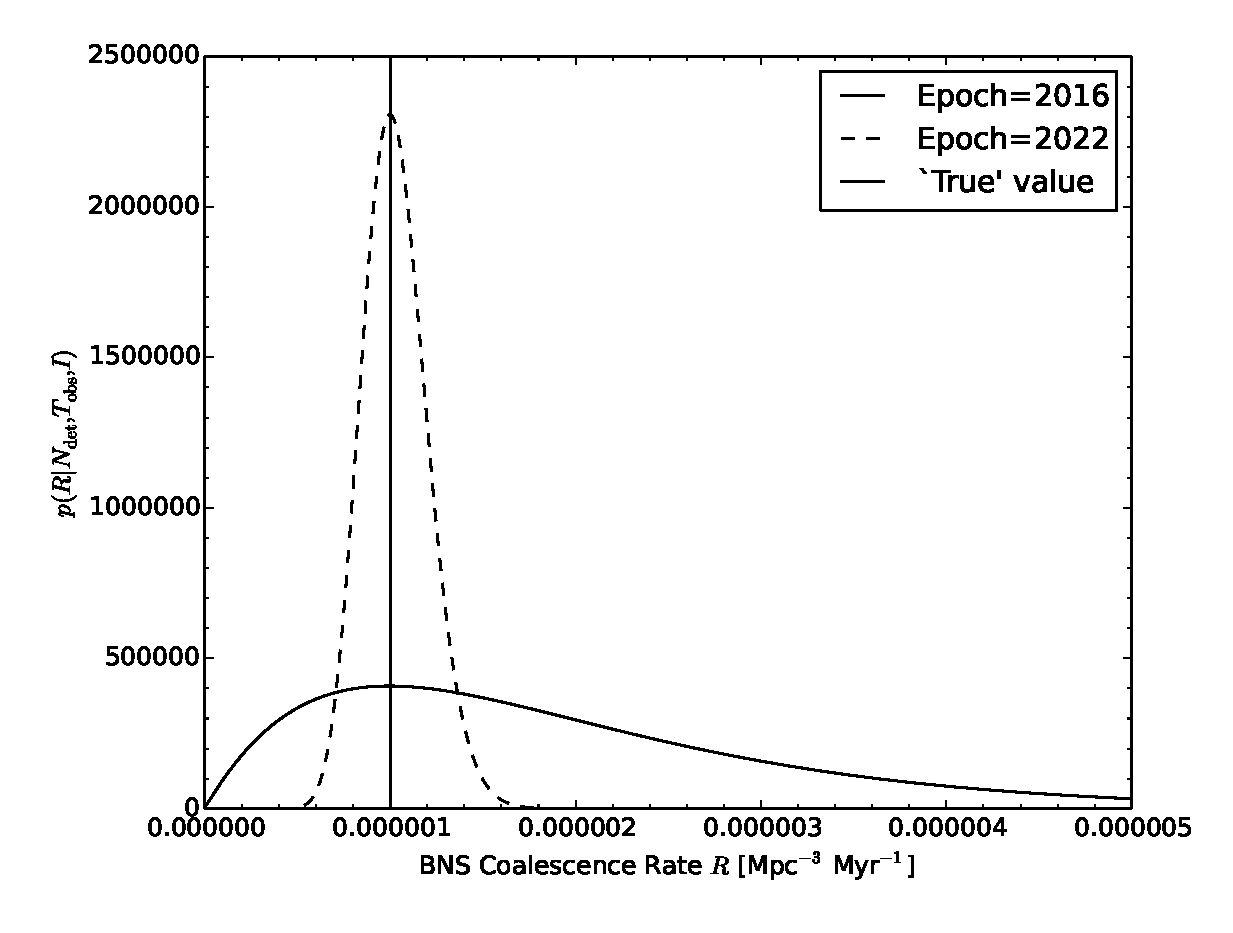
\includegraphics[width=\linewidth]{aligo_rate_re.eps}}
\caption{Posterior probability distribution for the rate of \bns{} coalescence
    assuming the 2016 (solid curve) \& 2022 (dashed curve) detection scenarios.
    These posteriors have been computed assuming a number of \gw{} inspiral
    detections commensurate with the `realistic' value
$\cbcrate=10^{-6}$\,Mpc$^{3}$yr$^{-1}$.  The 2022 epoch results in a greater
number of expected detections (40 vs 1.3), reducing the uncertainty in the
measurement.\label{fig:aligorate}}
\end{figure}

\subsubsection{Validation}
Before we go ahead and derive beaming angle posteriors corresponding to the
aforementioned observing scenarios, however, it is useful to establish some form
of validation for our procedure.  This validation is performed by first
selecting values of the beaming angle, say $\theta=30^{\circ}$; the \sgrb{}
efficiency, say $\epsilon=0.5$ and we use the `realistic' rate for the rate of
\bns{} coalescence $\cbcrate$.  We then compute the value of the \sgrb{} rate
which would correspond to these parameter choices.  Finally, we simply use this
\emph{artificial} value for $\grbrate$ in equation~\ref{eq:beam_posterior} when
we compute the posterior on the beaming angle on the understanding that the
resulting posterior should yield an inference consistent with the `true' value
$\theta=30^{\circ}$.
%
\begin{figure}%[H]
\centering
{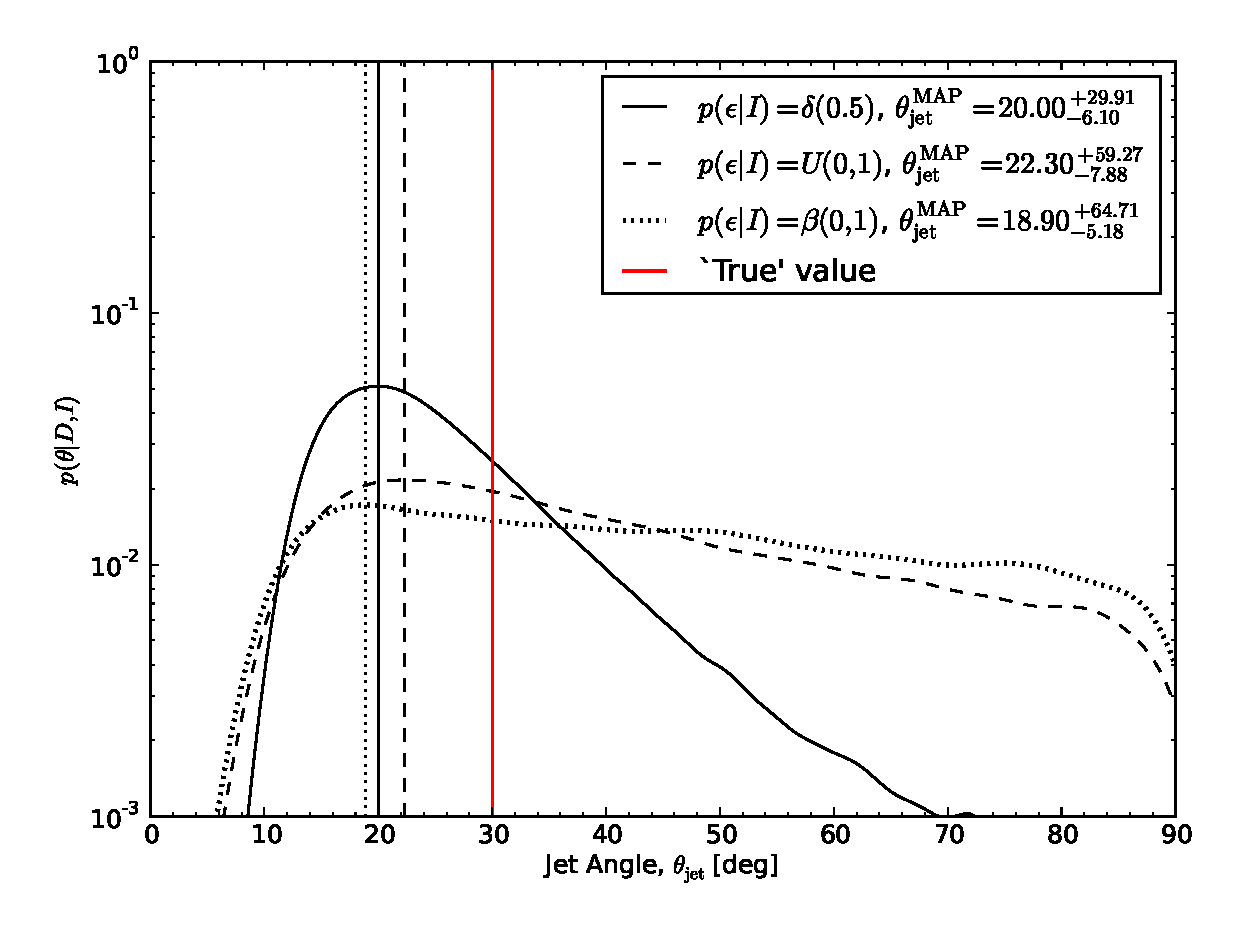
\includegraphics[width=\linewidth]{jet_angle_posterior_aligo_2016.eps}}
\caption{Beaming angle posteriors with different priors and where an artificial \sgrb{}
    rate has been imposed in order that the target value of the beaming angle is
$\theta = 30^{\circ}$.  These posteriors are based on the 2016 observing
scenario (see table~\ref{table:scenarios}). \label{fig:injjetposterio2016}}
\end{figure}
%
\begin{figure}%[H]
\centering
{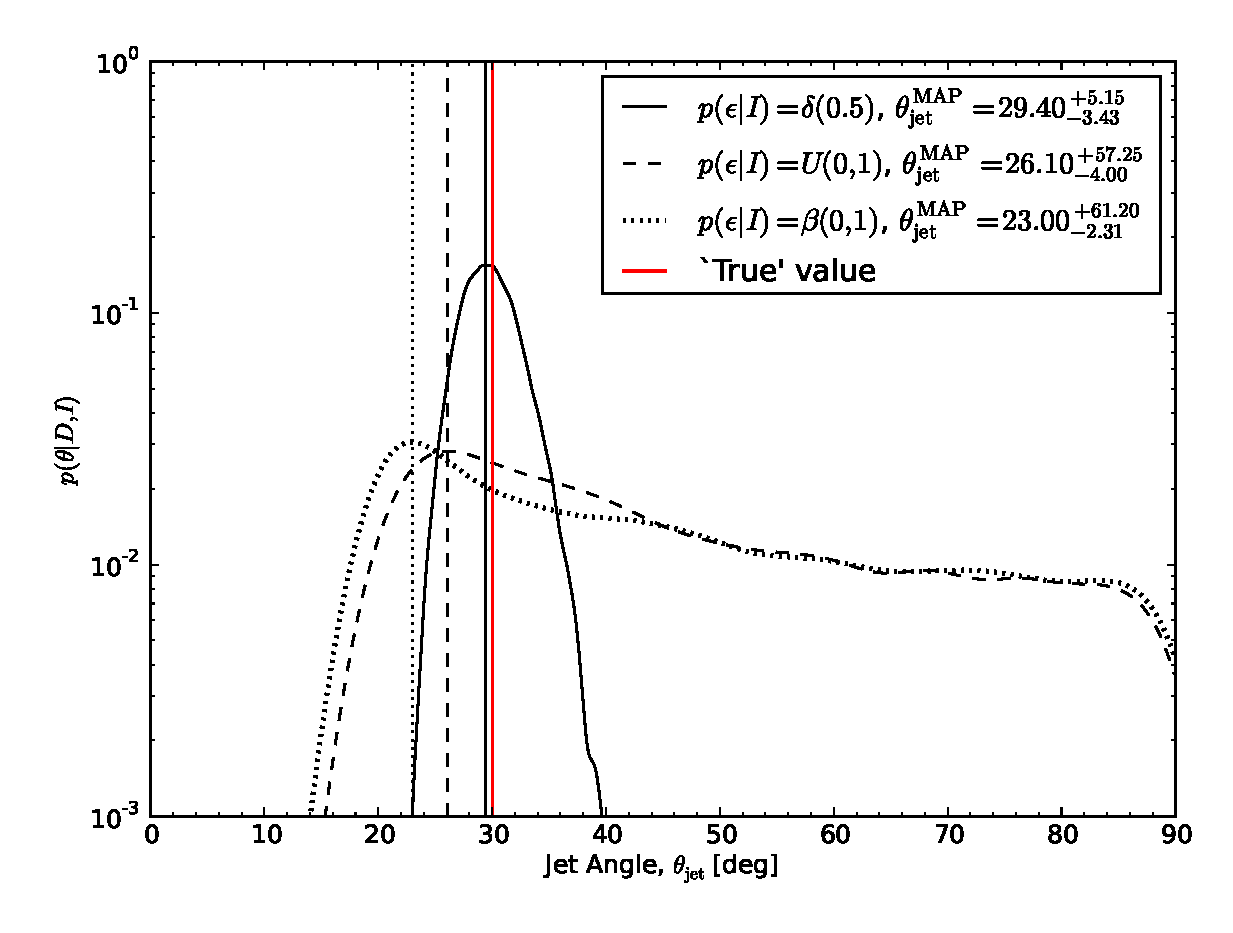
\includegraphics[width=\linewidth]{jet_angle_posterior_aligo_2022.eps}}
\caption{Beaming angle posteriors with different priors and where an artificial \sgrb{}
    rate has been imposed in order that the target value of the beaming angle is
$\theta = 30^{\circ}$.  These posteriors are based on the 2022 observing
scenario (see table~\ref{table:scenarios}). \label{fig:injjetposterio2022}}
\end{figure}
%
Figures~\ref{fig:injjetposterio2016} and~\ref{fig:injjetposterio2022} show the
beaming angle posteriors which result from this analysis for the 2016 and 2022
scenarios, respectively.  Unsurprisingly, the most accurate constraints arise
when we already have the tightest possible constraints on the \sgrb{} efficiency
$\epsilon$.  That is, the beaming angle posterior arising from the
$\delta$-function prior on $\epsilon$ is the narrowest, yielding the shortest
possible confidence interval.  It is well worth remembering, however, that had
we been incorrect regarding the value of $\epsilon$ when using the
$\delta$-function prior, the result would be significantly biased and our
inference on the beaming angle would be incorrect.  This highlights the
necessity of building a suitable representation of our ignorance into the
analysis.  Finally, we note that the results from the uniform and
$\beta$-distribution priors are broadly equivalent.


\subsubsection{Jet Angle Posteriors From Observing Scenarios}
Figures~\ref{fig:jetposterior2016} and~\ref{fig:jetposterior2022} show the
beaming angle posteriors obtained for our two detection scenarios.  Since it is
a common assumption in related literature, we also now include a prior on the
\sgrb{} efficiency which dictates that all \bns{} produce a \sgrb{},
$p(\epsilon|I)=\delta(\epsilon=1)$, as well as our previous strong
$\delta$-function prior.  For the 2016 scenario where inferences are somewhat
weak (i.e., broad posteriors) due to the sparcity of \gw{} detections, the
uncertainties are large enough that the results from each prior are broadly
consistent.  In the 2022 scenario, where the posterior is more peaked, it is
clear that the strong $\delta$-function priors lead to inconsistent inferences
on the \sgrb{} beaming angle.  The much weaker uniform and $\beta$
distributions, by contrast, are again largely consistent with each other
yielding more conservative and robust results, as well as being a more
representative expression of our state of knowledge.  The inferences drawn from
each scenario and each prior are summarised in terms of the maximum \emph{a
posteriori} measurement and the 90\% confidence interval around the maximum in
table~\ref{table:aligo_beam_inference}.

\begin{figure}
\centering
{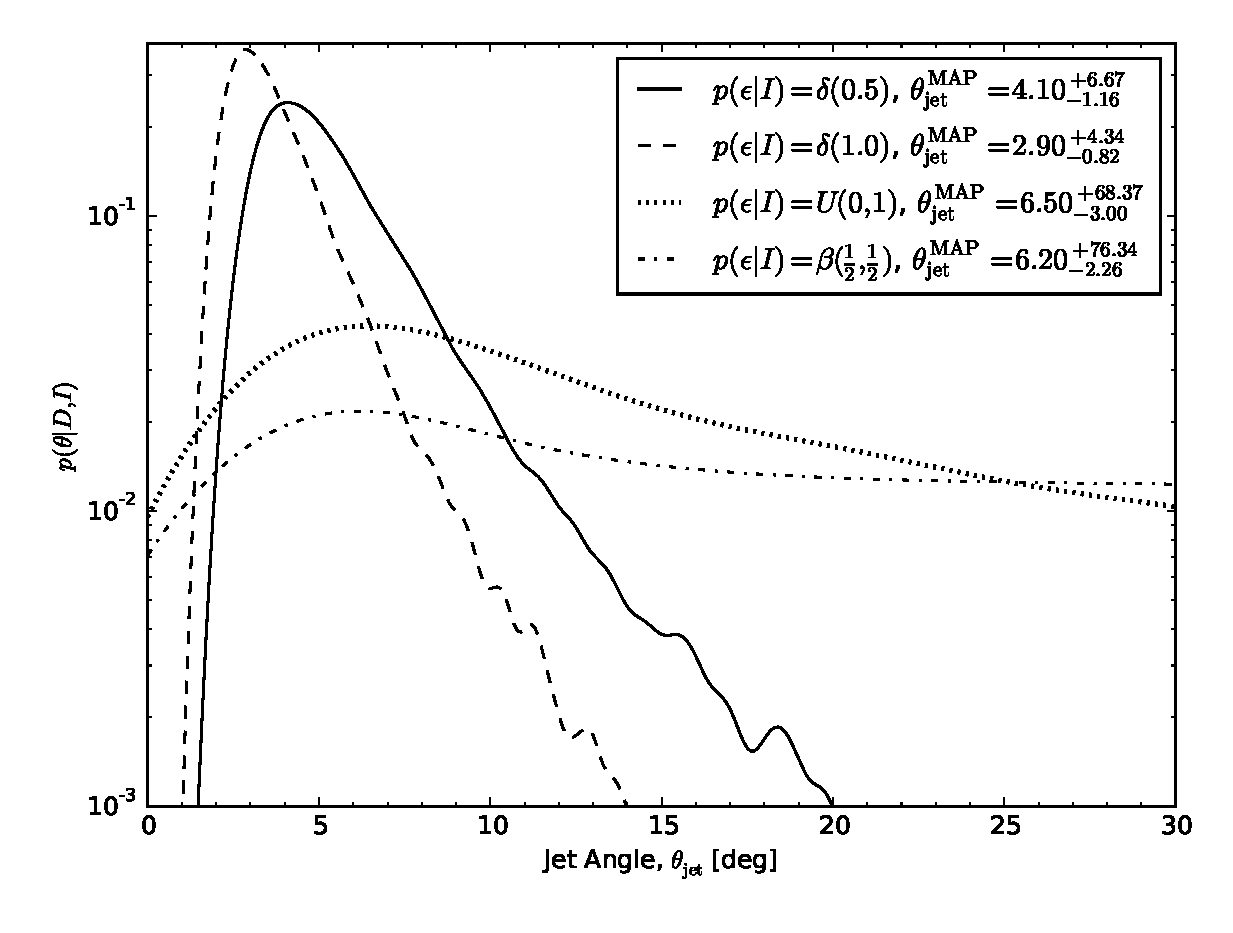
\includegraphics[width=\linewidth]{jet_angle_posterior_aligo_2016_re_real.eps}}
\caption{Beaming angle posteriors using different priors on \sgrb{} efficiency
$\epsilon$ in the 2016 observing scenario.\label{fig:jetposterior2016}}
\end{figure}

\begin{figure}
\centering
{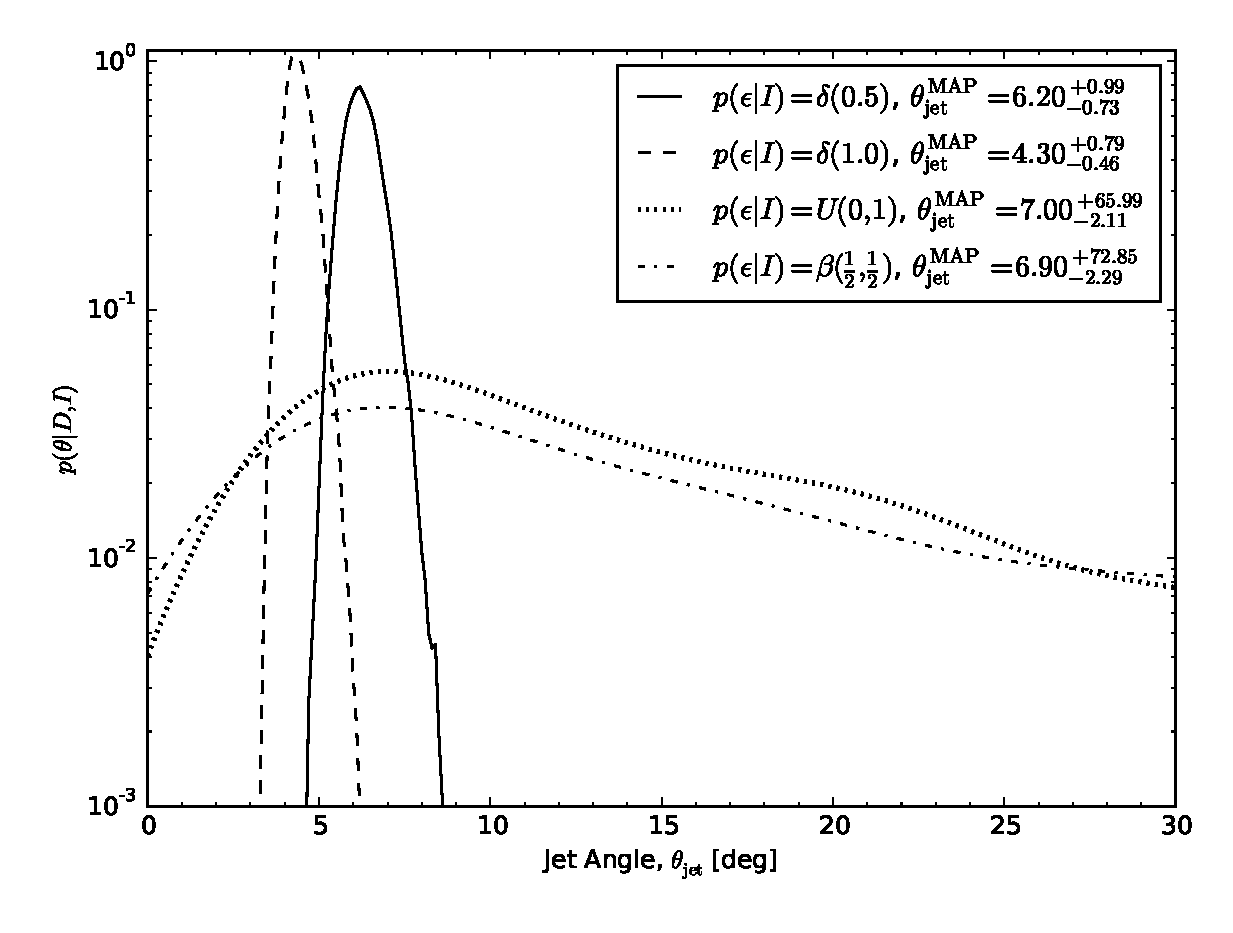
\includegraphics[width=\linewidth]{jet_angle_posterior_aligo_2022_re_real.eps}}
\caption{Beaming angle posteriors using different priors on \sgrb{} efficiency
$\epsilon$ in the 2022 observing scenario.\label{fig:jetposterior2022}}
\end{figure}

\begin{table}
\centering
\begin{tabular}{l c c c c }
\toprule
% &\multicolumn{4}{c}{Prior} \\
Scenario & $\delta(\epsilon=0.5)$ & $\delta(\epsilon=1)$ & $U(0,1)$ & $\beta(\frac{1}{2},\frac{1}{2})$\\
\cline{1-1}\cline{2-5}
\colrule
2016  & $4.10^{+6.67}_{-1.16}$ & $2.90^{+4.34}_{-0.82}$ &\ $6.50^{+68.37}_{-3.00}$ & $6.20^{76.34}_{-2.26}$ \\
2022 & $6.20^{+0.99}_{-0.73}$ & $4.30^{+0.79}_{-0.46}$ & $7.00^{+65.99}_{-2.11}$ & $6.90^{+72.85}_{-2.29}$ \\
\botrule
\end{tabular}
\caption{Summary of the beaming angle inferences for each prior in the two
observing scenarios considered in this work.  Point estimates are the maximimum
a posteriori estimates and errors correspond to the $90\%$ confidence interval
around the maximum.\label{table:aligo_beam_inference}}
\end{table}

%   \begin{figure}
%   \centering
%   {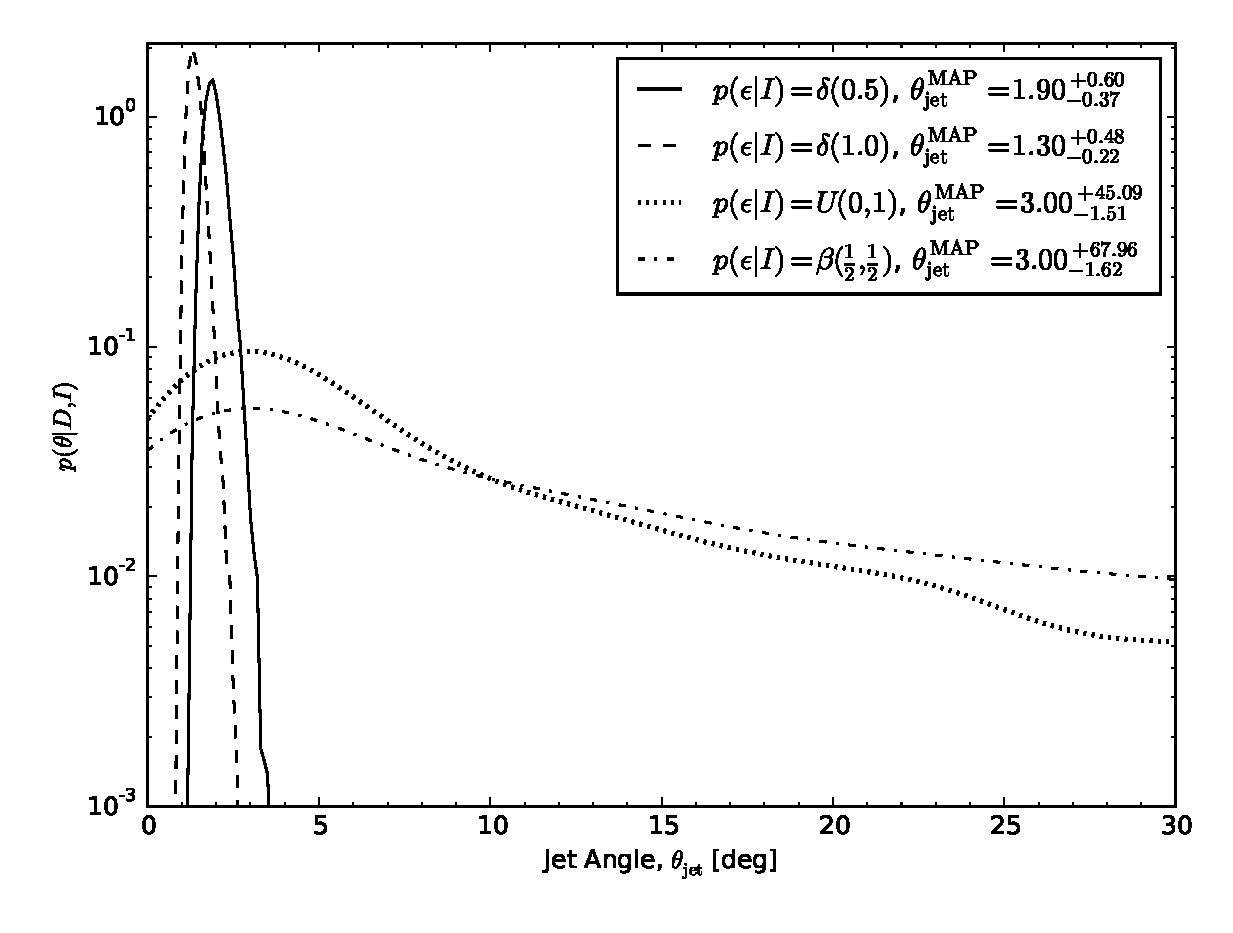
\includegraphics[width=\linewidth]{jet_angle_posterior_aligo_2016_high_real.eps}}
%   \caption{ADE 2016 jet angle posterior, high rate}
%   \end{figure}
%
%   \begin{figure}
%   \centering
%   {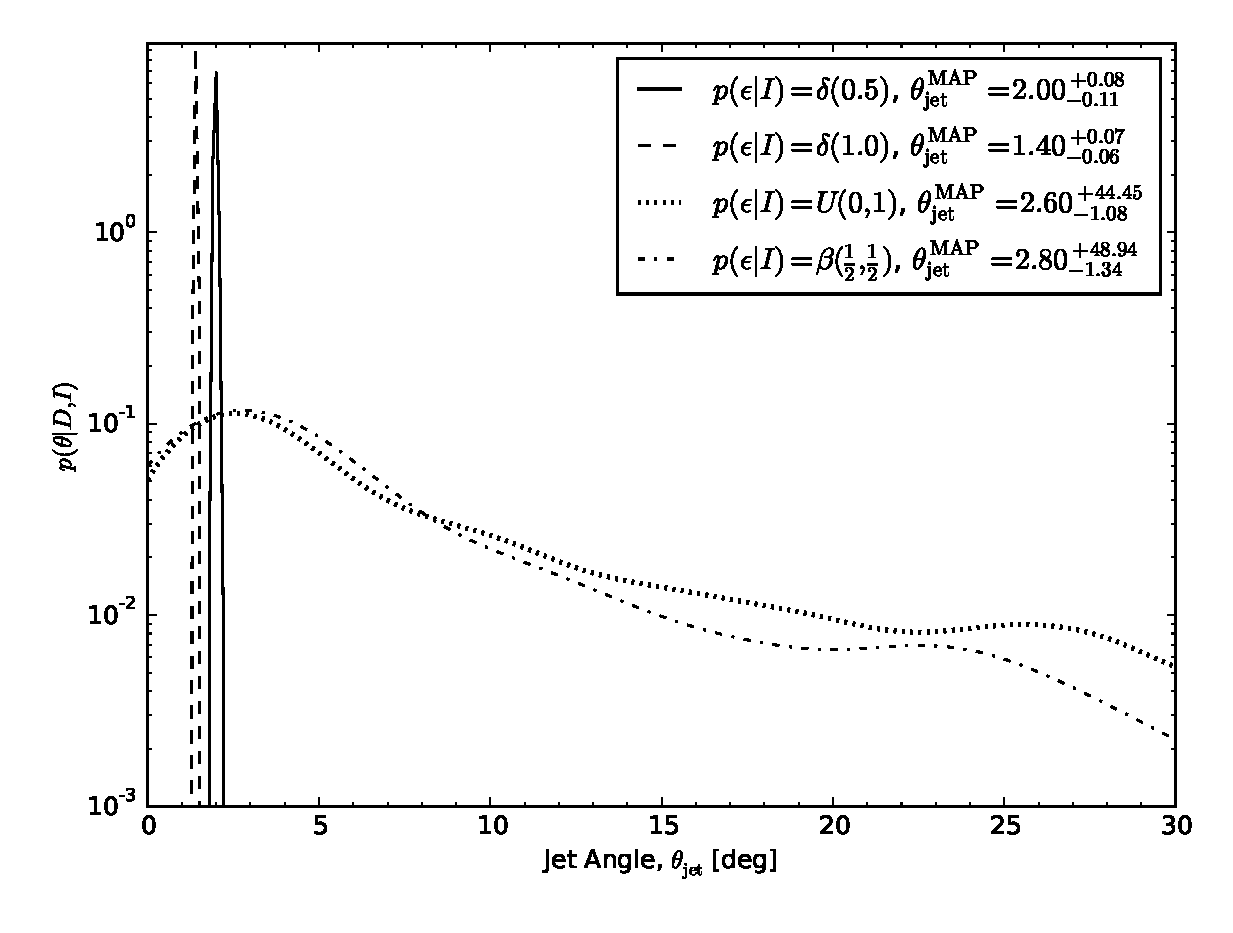
\includegraphics[width=\linewidth]{jet_angle_posterior_aligo_2022_high_real.eps}}
%   \caption{ADE 2022 jet angle posterior, high rate}
%   \end{figure}

\section{Beaming Angle Constraints With No \gw{} Detections}
\label{sec:beaming_limits}
Our proposed approach is also valid in the regime where no gravitational wave
signals from \bns{} coalescence have been observed and the procedure is
identical: construct the posterior probability density function on the \bns{}
coalescence rate, transform to the joint posterior on the beaming angle and
\sgrb{} efficiency $\epsilon$ and marginalise over the nuisance parameter
$\epsilon$ to yield the posterior on the beaming angle.  Now, however, rather
than quoting (say) the maximum a posteriori estimate, together with some
confidence interval, we simply integrate the beaming angle posterior from
$\theta=0$ until we reach that value which contains some desired confidence.
Thus, we obtain an upper limit on the beaming angle, analogous to the rate upper
limits set by past LIGO observations~\cite{S6lowmass}.

In this section, we demonstrate the procedure using the \bns{} coalescence rate
measurements from the final science run of LIGO, prior to the upgrade to aLIGO.

\subsection{Constructing The Rate Posterior}
Our first objective is the construction of the rate posterior.  Since our
ultimate goal here is to derive a beaming angle posterior based on initial LIGO
observations, it is convenient to adopt the same approach to constructing the
rate posterior that was used in past analyses.
Following~\cite{Biswas09,BradyFairhurst08}, the posterior on the binary
coalescence rate may be determined from the loudest event in the \gw{} analysis
and takes the form,
%Specifically, for a foreground event rate due to  binary coalescence $\cbcrate$,
%the probability of obtaning no events with ranking statistic $\rho$ greater than
%the observed loudested event $\rhostar$ is,
%
%\begin{equation}
%P_F(\rhostar | \cbcrate, C_L, T) = e^{-\cbcrate C_L(\rhostar) T},
%\end{equation}
%
%where $C_L(\rhostar)$ is the total luminosity to which the search is sensitive
%and $T$ is the duration of the search.  The overall probability of obtaining
%no events with ranking statistic $\rho>\rhostar$ is the product of obtaining
%no such events from foreground \emph{and} the probability of obtaining no such
%events from the background in the detector, denoted $P_B(\rhostar)$,
%
%\begin{equation}
%P(\rhostar|\cbcrate,I) = P_B(\rhostar|I)e^{-\cbcrate C_L(\rhostar) T}
%\end{equation}
%
%Using a uniform prior on $\cbcrate$ and inverting the overall probability with
%Bayes' theorem, we arrive at,
%
\begin{equation}\label{eq:loudestEventPosterior}
p(\cbcrate | C_L({\rhostar}), T, \Lambda) \propto p(\cbcrate) \left[ \frac{1+\Lambda
C_L(\rhostar) T}{1+\Lambda}\right] e^{-\cbcrate C_L(\rhostar) T},
\end{equation}
%
where $p(\cbcrate)$ is the prior probability distribution on the rate, assumed
to be uniform; $C_L(\rhostar)$ is the total luminosity to which the search is
sensitive and $T$ is the observation time.  The quantity $\Lambda$ is
essentially the relative likelihood that the loudest event arose from a \gw{}
signal to the likelihood of background.  The reader is directed to section\,3
of~\cite{BradyFairhurst08} for the derivation of this distribution and the
quantities involved.

We can now use the published upper limits on the rate of \bns{} coalescence to
re-derive the full rate posterior.  The upper limit on the binary coalescence
rate at confidence $\alpha$ is found by integrating the rate posterior from zero
to $\alpha$.  Assuming a uniform prior on the rate $\cbcrate$ and using the rate
posterior given by equation~\ref{eq:loudestEventPosterior}, the upper limit on
the rate $\cbcrate_{\alpha}$ is given by equation 21 in~\cite{BradyFairhurst08}:
%
\begin{equation}
1-\alpha =  e^{-\cbcrate_{\alpha} C_L(\rhostar)T)}
\left[ 
1+ \left(\frac{\Lambda}{1+\Lambda}\right) \cbcrate_{\alpha} T C_L(\rhostar)
\right ].
\label{eq:rateIntegral}
\end{equation}
%
In the event that no \gw{} signal has been observed and the loudest event is
umabiguously due to background noise fluctuations, we are in the limit in which
$\Lambda \rightarrow 0$.  In this case, we simply have,
\begin{equation}
C_L(\rhostar)T = -\frac{\log(1-\alpha)}{\cbcrate_{\alpha}},
\end{equation}
%
%and the value of $\cbcrate$ can be taken straight from the literature
%\footnote{Note
%that this procedure necessarily confines our jet angle inferences based on
%progenitor systems for which the rate upper limits are available.  Given that
%the binary coalesence rate limits are quoted for canonical binary neutron star
%and neutron star-black hole systems, both plausible sGRB progenitors, this
%simply means our inferences on the jet angle are specific to each system and
%treated separately.}
%

\begin{figure}
\centering
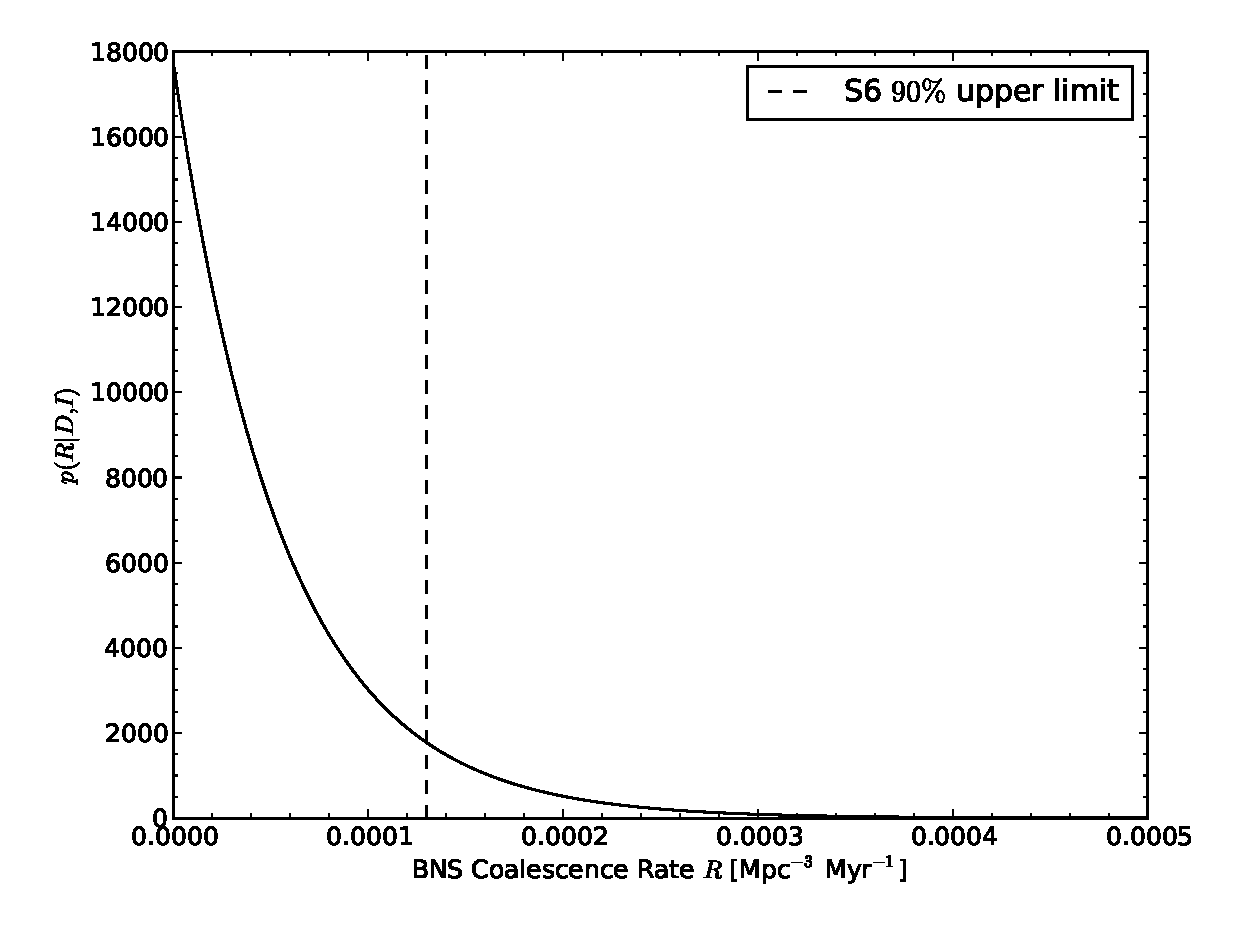
\includegraphics[width=\linewidth]{S6_rate.eps}
\caption{Posterior on the rate of \bns{} coalescence based on obsevations taken
    during the S6/VSR2,3 science runs of initial LIGO and
    Virgo~\cite{S6lowmass}. The posterior is constructed using the loudest event
    procedure~\cite{Biswas09,BradyFairhurst08} and reconstructed from published
upper limits (see text).\label{fig:s6rate}}
\end{figure}

Using the most stringent 90\% confidence upper limit from \gw{} observations on
the rate of binary neutron star coalescences to date, $\cbcrate^{90\%}_{{\rm
bns}} = 1.3\times 10^{-4}$\,Mpc$^{-3}$yr$^{-1}$~\cite{S6lowmass}, gives
$C_L(\rhostar)T=17712$.  The full rate posterior from~\cite{S6lowmass} is then
found by inserting this value and $\lambda=0$ in
equation~\ref{eq:loudestEventPosterior}.  The result is shown in
figure~\ref{fig:s6rate}.


%Similarly, for NS-BH systems,  $\cbcrate^{90\%}_{{\rm
%nsbh}} = 3.1\times 10^{-5}$\,Mpc$^{-3}$yr$^{-1}$ gives $C_L(\rhostar)T=74277$.
%The posteriors on the rates, assuming these values and $\Lambda=0$, are shown in
%figure~\ref{fig:reconstructedRatePosterior}.  

\subsection{Results}
Figure~\ref{fig:s6angle} shows the four posteriors on the beaming angle,
corresponding to the four priors on the grb efficiency $\epsilon$, using the
rate posterior obtained from \gw{} measurements in the final science run of the
first generation of ground based \gw{} detectors.  In this null-detection
scenario, we choose to compute the 95\% confidence \emph{upper} limit on the
beaming angle,
\begin{equation}
    \label{eq:beaming_upper_limit}
    0.95 = \int_0^{\theta^{\mathrm{ul}}} p(\theta|D,I)~\diff \theta
\end{equation}
%
We see that here, where the rate posterior is rather uninformative, the results
are dominated by the uncertainty in $\epsilon$: there are substantive
differences in the beaming angle upper limits yielded by the uniform ($U(0,1)$)
and $\beta$-distribution priors, while the $\delta$-function priors yield
dramatically different upper limits.  Indeed, the most stringent (and mutually
incompatible) upper limits are obtained using the strong $\delta$-function
priors.  In fact, these beaming angle upper limits are also incompatible with
the values of $3^{\circ}\mbox{-}8^{\circ}$ that have been inferred from
observations of jet breaks in \sgrb{} afterglows~\cite{2014ApJ...780..118F,
2006MNRAS.367L..42P, 2012A&A...538L...7N}.  Recall, however, from the discussion
in section~\ref{sec:sgrbs} that we interpret the beaming angle inference from
our rate measurements as the upper bound on the mean of a population of beaming
angles.  It would, therefore, seem premature to conclude that there is tension
in these results; instead, we can only state that either the population of
\sgrb{s} have a distributio of beaming angles with some finite width or that the
fraction of \bns{} mergers which yield a \sgrb{} is smaller than 0.5.

It is also interesting to compare these upper limits on the beaming angle with
those in~\cite{2013PhRvL.111r1101C}, where the upper limit on the rate itself is
used as a constraint (rather than transforming the posterior).  This has the
important implication that the constraint thus obtained is the \emph{smallest}
angle consistent with the rate:
%
\begin{equation}
    1 - \cos \theta \geq \frac{\grbrate}{\epsilon \cbcrate^{\mathrm{ul}}},
\end{equation}
%
where $\cbcrate^{\mathrm{ul}}$ is the \emph{upper limit} on the \bns{} rate.
The same idea is used in~\cite{0004-637X-809-1-53} to estimate beaming
constraints in the advanced detector era.  Thus, when comparing the constraints
in e.g.,~\cite{2013PhRvL.111r1101C} and the upper limits obtained from the
transformed posterior (i.e., equation~\ref{eq:beam_posterior} and
figure~\ref{fig:s6angle}), one should remember that they are quite different
quantities.  There are two other noteworthy differences
between~\cite{2013PhRvL.111r1101C} and this work: (i) the rate upper limit is
computed based on the sensitivity of the initial LIGO/Virgo network (see
e.g.,~\cite{BradyFairhurst08}), which gives $\cbcrate=4.5\times
10^{-4}$\,Mpc$^{-3}$yr$^{-1}$ (as compared with $\cbcrate=1.3 \times
10^{-4}$\,Mpc$^{-3}$yr$^{-1}$ from the analysis in~\cite{S6lowmass}) and (ii) it
is implicitly assumed that \emph{all} \bns{} mergers yield an \sgrb{}.  That is,
there is no factor or $\epsilon$ to account for the unknown fraction of mergers
which successfully launch a \grb{} jet.  With these differences noted, the lower
bound on the beaming angle is found to be $\theta \geq 0.8^{\circ}$, as compared
with our 95\% confidence upper limit $\theta^{\mathrm{ul}}=1.94^{\circ}$ when
assuming $\epsilon=1$.  

\begin{figure}
\centering
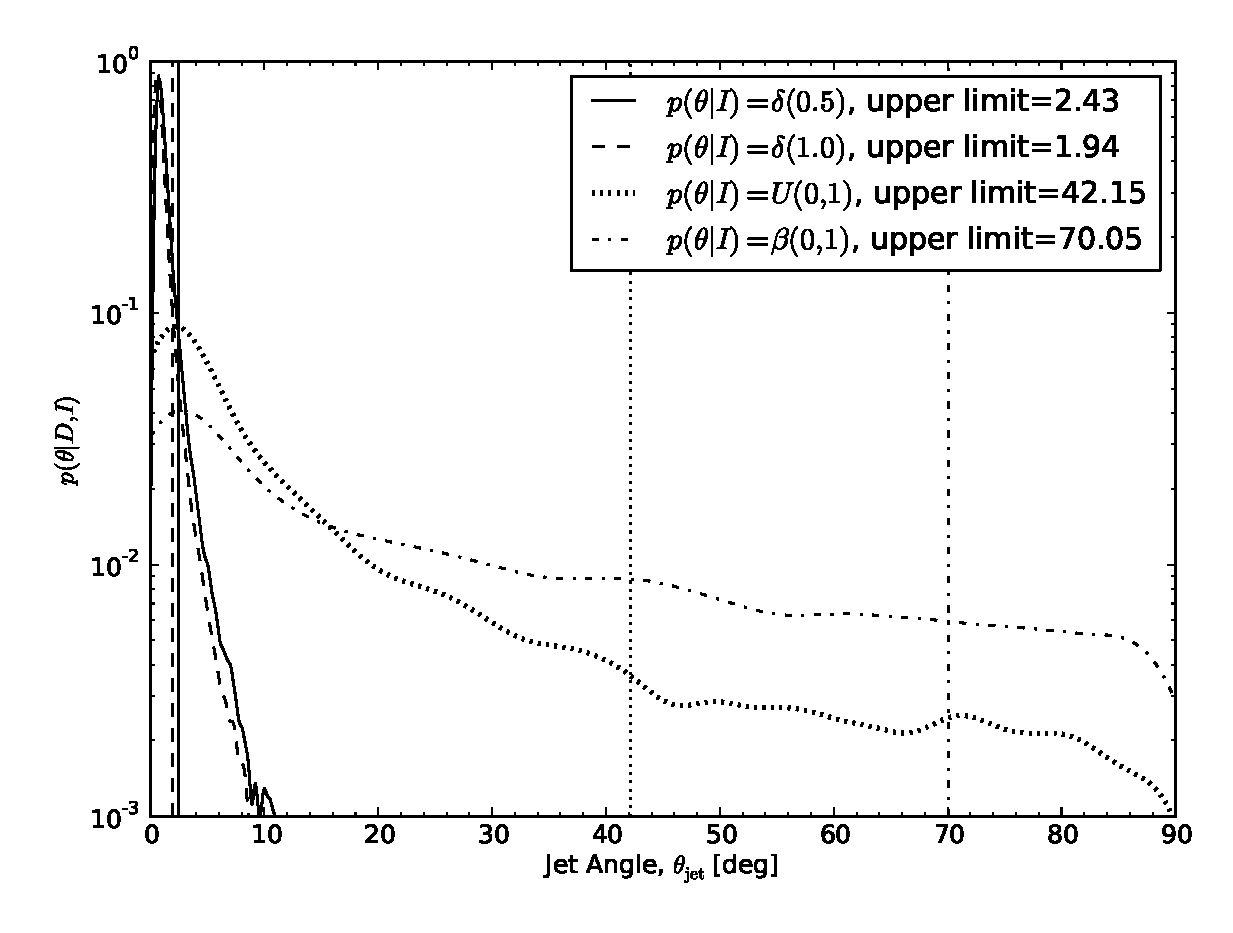
\includegraphics[width=\linewidth]{jet_angle_posterior_iligo.eps}
\caption{Beaming angle posterior using the rate posterior (see
figure~\ref{fig:s6rate}) obtained from S6/VSR2,3 observations~\cite{S6lowmass}.
Priors on $\epsilon$ now dominate our results.\label{fig:s6angle}}
\end{figure}

\section{Conclusion}

\begin{comment}

\appendix


\section{Jacobian Calculation}
This doesn't need to be in the publication, these are just notes for James'
benefit and possibly verification.

\begin{equation}
\cbcrate=\frac{\grbrate}{\epsilon(1-\cos \theta)},
\end{equation}

\begin{equation}
p(\theta) = \int_{\epsilon} p(\theta,\epsilon)~\diff \epsilon,
\end{equation}

\begin{equation}
p(\theta,\epsilon) = p(\cbcrate,\epsilon)
\left\lvert\left\lvert
\frac{\partial(\cbcrate,\epsilon)}{\partial(\theta,\epsilon)}
\right\rvert\right\rvert,
\end{equation}

% Increase matrix line spacing
\begingroup
\renewcommand*{\arraystretch}{1.5}

% matrix:
\begin{equation}
\frac{\partial (\cbcrate,\epsilon)}{\partial(\theta,\epsilon)} =
\begin{bmatrix}
\frac{\partial \cbcrate}{\partial \theta} & \frac{\partial \cbcrate}{\partial \epsilon} \\
\frac{\partial \epsilon}{\partial \theta} & \frac{\partial \epsilon}{\partial \epsilon}
\end{bmatrix}.
\end{equation}

% end line spacing increase
\endgroup

\begin{eqnarray}
\frac{\partial \cbcrate}{\partial \theta} & = &
-\frac{\grbrate\sin\theta}{\epsilon(\cos\theta - 1)^2}\\
\frac{\partial \cbcrate}{\partial \epsilon} & = &
\frac{\grbrate}{\epsilon^2(\cos\theta-1)}\\
\frac{\partial \epsilon}{\partial \theta} & = &
-\frac{\grbrate\sin\theta}{\cbcrate(\cos\theta-1)^2}\\
\frac{\partial \epsilon}{\partial \epsilon} & = & 1\\
\end{eqnarray}

\begin{eqnarray}
\left\lvert
\frac{\partial(\cbcrate,\epsilon)}{\partial(\theta,\epsilon)}
\right\rvert & = & \frac{\partial \cbcrate}{\partial \theta}
\frac{\partial \epsilon}{\partial \epsilon} - \frac{\partial \cbcrate}{\partial
\epsilon}\frac{\partial \epsilon}{\partial \theta} \\
& = & -\frac{2\sin\theta}{\epsilon(\cos\theta-1)^2}
\end{eqnarray}
%
Finally:
\begin{equation}
\left\lvert\left\lvert
\frac{\partial(\cbcrate,\epsilon)}{\partial(\theta,\epsilon)}
\right\rvert\right\rvert = \frac{2\grbrate\sin\theta}{\epsilon(\cos\theta-1)^2} 
\end{equation}

\section{Null-detection Jet Angle Posteriors With Different Priors}

\end{comment}

\bibliography{grb_beams_paper}

\end{document}
